% CVPR 2023 Paper Template
% based on the CVPR template provided by Ming-Ming Cheng (https://github.com/MCG-NKU/CVPR_Template)
% modified and extended by Stefan Roth (stefan.roth@NOSPAMtu-darmstadt.de)

\documentclass[10pt,twocolumn,letterpaper]{article}

%%%%%%%%% PAPER TYPE  - PLEASE UPDATE FOR FINAL VERSION
\usepackage[final]{cvpr}      % To produce the REVIEW version
%\usepackage{cvpr}              % To produce the CAMERA-READY version
%\usepackage[pagenumbers]{cvpr} % To force page numbers, e.g. for an arXiv version

% Include other packages here, before hyperref.
\usepackage{graphicx}
\usepackage{amsmath}
\usepackage{amssymb}
\usepackage{booktabs}
\usepackage{adjustbox}


% It is strongly recommended to use hyperref, especially for the review version.
% hyperref with option pagebackref eases the reviewers' job.
% Please disable hyperref *only* if you encounter grave issues, e.g. with the
% file validation for the camera-ready version.
%
% If you comment hyperref and then uncomment it, you should delete
% ReviewTempalte.aux before re-running LaTeX.
% (Or just hit 'q' on the first LaTeX run, let it finish, and you
%  should be clear).
\usepackage[pagebackref,breaklinks,colorlinks]{hyperref}


% Support for easy cross-referencing
\usepackage[capitalize]{cleveref}
\crefname{section}{Sec.}{Secs.}
\Crefname{section}{Section}{Sections}
\Crefname{table}{Table}{Tables}
\crefname{table}{Tab.}{Tabs.}


%%%%%%%%% PAPER ID  - PLEASE UPDATE
\def\cvprPaperID{*****} % *** Enter the CVPR Paper ID here
\def\confName{CVPR}
\def\confYear{2022}


\begin{document}

%%%%%%%%% TITLE - PLEASE UPDATE
\title{Applying Pose Estimation to Predict the Outcome of A Free Throw}

\author{Laith Altarabishi\\
University of Texas at Austin\\
{\tt\small laithaustin@utexas.edu}
% For a paper whose authors are all at the same institution,
% omit the following lines up until the closing ``}''.
% Additional authors and addresses can be added with ``\and'',
% just like the second author.
% To save space, use either the email address or home page, not both
\and
Sidharth Babu\\
University of Texas at Austin\\
{\tt\small sidharth.n.babu@utexas.edu}
\and
Afnan Mir \\
University of Texas at Austin\\
{\tt\small afnanmir@utexas.edu}
\and
Zayam Tariq \\
University of Texas at Austin\\
{\tt\small zayamtariq@utexas.edu}
}
\maketitle

%%%%%%%%% ABSTRACT
\begin{abstract}
  In this report, we present an end-to-end pipeline that includes a pose estimator as well as 
  a classification model that can effectively predict the outcome of a free throw. Our training data was
  self-generated by recording hundreds of clips of our test subject shooting free throws of various forms
  and recording the outcome. We explore different ways to generate feature vectors for inputs to our model as 
  well as multiple classification models to produce the best performing pipeline. Our code can be found \href{https://github.com/afnanmmir/Shot-Predictor/}{here}.
\end{abstract}


%%%%%%%%% BODY TEXT
\section{Introduction}
\label{sec:intro}

In basketball, the ability of a player to effectively shoot the basketball typically comes down to the player’s shooting form. While the form of the best shooters tend to look different, they all typically use the same fundamentals. In our project, we will attempt to capture these fundamental aspects of a player’s shooting form and attempt to predict the outcome of a shot using these features. Research has been done on extracting features from a player’s movement to classify the action a player is performing (shooting, dribbling, etc.) \cite{Basketball}, but we would like to focus our energy on feature extraction from the shooting motion using pose estimation \cite{OpenPose}, object detection \cite{YOLO}, and possibly other methods to extract feature descriptors of a shot and attempt to identify it as a make or a miss.\\
\indent This problem is a particularly nontrivial application of pose estimation for two main reasons. The first being that there are multiple stages to
a basketball shot that need to be taken into account. From dipping the ball to waist level, to the motion of bringing the ball to eye level, to releasing the ball, each
plays a significant role in the outcome of a shot, so each stage needs to be taken into account. The second reason is the variability of the average shot. It can be argued that no two shots will ever be identical due to the imperfect nature of humans.
Therefore, it is necessary for our feature representation of a shot to be invariant towards miniscule changes
in shot form and focus more on fundamental differences.
%-------------------------------------------------------------------------
%------------------------------------------------------------------------
\section{Related Works}
\label{sec:formatting}

%-------------------------------------------------------------------------
\subsection{Pose Estimation}

Pose Estimation is a critical topic in computer vision that will intersect with our goal of trying to accurately capture the motion and actions of a person taking a shot in basketball. Pose estimation, in the context of 2D videos of humans, is the problem of localizing anatomical keypoints or joints in a frame by frame video or image \cite{OpenPose}. To fulfill our goal of predicting the outcome of a basketball shot, it will be critical to assess the form of a player who's taking a shot - where form can be decomposed into various classifications of joints in space. Pose estimation methods can be categorized into bottom-up or top-down methodologies. Bottom-up methodologies start by estimating keypoints and body joints first, and then these points are clustered to form poses. In contrast, 
top-down methodologies of pose estimation first run a person detector before decomposing each person into their respective body joints within detected bounding boxes \cite{Viso2}. Computational complexity is a major consideration for landmark pose estimation algorithms, and modern SOTA pose estimation algorithms deploy deep learning and CNNs to improve compuational overhead and speed \cite{OpenPose}. We list some examples of prevalent and SOTA pose estimation models that have been employed and researched below.
%
\begin{quotation}
  OpenPose: The first multi-person realtime 2D pose estimation system that uses a bottom-up approach that implements nonparametric representation to associate human keypoints and body parts with an individual in an image \cite{OpenPose}. \\
  \newline
  \indent DeepPose: SOTA pose estimation method that uses DNNs to classify human body joints through the usage of cascading DNN regressors that produce high precision pose estimates \cite{DeepPos}. \\
  \newline
  \indent AlphaPose: Multi-person SOTA realtime pose estimation system that outperforms OpenPose in AP score and has a high mAP score \cite{Alpha}. \\
  \newline
  \indent DeepCut: Proposes an approach to solving issues in both pose estimation and detection by using a partitioning and labeling formulation of a set of CNN part detectors \cite{DeepCut}.
\end{quotation}

Pose estimation attempts to detect the location of 17 keypoints on a human body, as seen in Figure \ref{fig:pose}. These keypoints include key joints such as
the knee, elbow, shoulder, and wrist, which can be vital in determining the form of a free throw.
\begin{figure}[h]
  \centering
  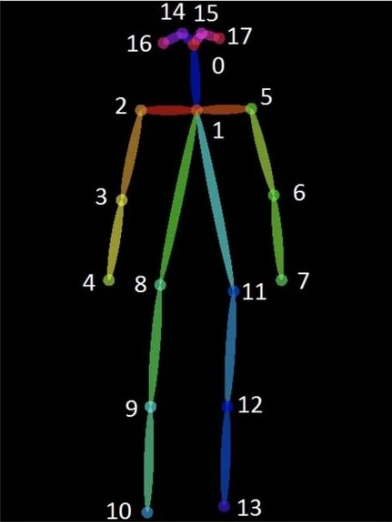
\includegraphics[width=0.25\textwidth]{imgs/openpose.png}
  \caption{Pose estimation keypoints}
  \label{fig:pose}
\end{figure}
%
 
%-------------------------------------------------------------------------
\subsection{Basketball and Pose Estimation}

The application of pose estimation in basketball is not a new concept. Collecting and analyzing basketball player's
posture data is an important facet of the scientific basketball community in order to help maximize training outputs.
For example, pose estimation was used in combination with classification models to predict the action a player is performing
in a video \cite{Basketball}. This is fairly similar to our project because it attempts to create feature vectors in video frames
using pose estimation to encode data about the motion of a player and use these features to make a prediction. However, our project
solely focuses on the motion of a player's shooting form and predicting the outcome of the shot.

%

%-------------------------------------------------------------------------
\subsection{Object Detection}

Our project will hope to capture and detect objects in high frame-rate video, with minimal computational overhead so that we are able to best assess the keypoints/human joints of our basketball shooters. 
In recent years, object detection algorithms have evolved greatly and most SOTA models today utilize deep learning to provide more robust results \cite{Viso}. There are many pre-existing SOTA object detection methods that have been utilized in the context of pose estimation methods and regression issues, and the following works are examples of some of them.

\begin{quotation}
  YOLO: Single stage object detection algorithm that frames detection as a regression problem to spatially seperated bounding boxes and associated class probabilities \cite{YOLO}.\\
  \newline
  \indent Mask R-CNN: Two-stage object detection algorithm that detects objects in an image while creating high-quality segmentation masks for each instance \cite{PatternRec}.\\
  \newline
  \indent Feature Pyramid Networks: Two-stage object detection algorithm that uses the multi-scale, pyramidial hierarchy of deep convolutional networks to create feature pyramids \cite{FeaturePyr}. \\
\end{quotation}

%------------------------------------------------------------------------
\section{Methodology}
\subsection{General Overview}
% We will have a camera taking in video input of a player shooting the basketball, potentially from two different angles.
% One angle would be a side view of the shooter that can capture the relative positions of the shooter and the hoop, and the other
% would be a head-on view of the of the shooter to capture the full pose estimation of the shooter.

% In the background, we will have our pose estimation algorithm running to capture the pose estimation of the shooter which will be used
% to make our predictions. Additionally, we will potentially be retrieving other data to create our feature vector, including the angle relationship
% between the shooter and the hoop, and the speed of the shot. We will be attempting to capture the pose estimation at multiple stages of the
% shot, as each stage can have a significant impact on the outcome of the shot. We will then take this feature vector and put it through a classification model.
% We will perform binary classification and predict whether a shot will go in or not.
The high-level overview of our end-to-end pipeline is shown in Figure \ref{fig:flowchart}. We start off by capturing clips of a test subject shooting a free throw. This will be our 
original data. We first want to downsample the video as we assume that many of the frames will be redundant and take up unnecessary computation time. After this, we perform pose estimation
on all the frames of each video to get the keypoints of our test subject for each video clip. Using the pose estimation data, we perform
feature extraction to generate feature vectors for each video clip according to some convention. This will be elaborated on in a later section. 

These feature vectors will be the training and testing data that we use for our classification model. We will want to split this data into training
and testing sets. We will train our classification model on the training set and generate predictions using our testing set.
\begin{figure}[h]
  \centering
  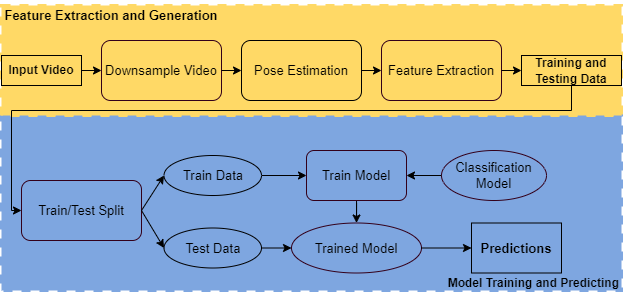
\includegraphics[width=0.45\textwidth]{imgs/cv_pipeline_real.png}
  \caption{Overview of Pipeline}
  \label{fig:flowchart}
\end{figure}

\subsection{Data Collection}
To fit the scope of our project, we wanted the shot data be as controlled as possible to prevent unwanted variations
in our data. To do this, we collected our own data, where we had our test subject always shoot from the free throw line
and had a camera in a fixed position in front of the test subject to capture their form. The set up can be seen in Figure \ref{fig:ft_data}.
We genereated approxiamately 300 clips of our test subject shooting free throws. Additionally, for this project, we wanted to detect major changes
in shooting forms that could affect the outcome of a shot. Therefore, our test subject shot some of their shots as he normally would, with the intent
of making it, and some of their shots with purposefully bad form, with the intent of missing. We had a relatively even split of these two types of shots. 

\begin{figure}
  \centering
  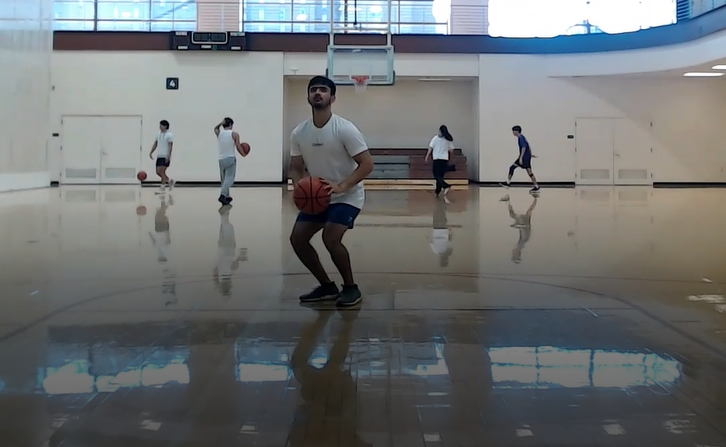
\includegraphics[width=0.45\textwidth]{imgs/data_collection.png}
  \caption{Free Throw}
  \label{fig:ft_data}
\end{figure}

\subsection{Pose Estimation}
For our pose estimation, we decided between using OpenPose and MoveNet pose estimators. These are both bottom up approaches to pose estimation. We decided on using bottom up pose estimators as this is the
current state of the art, and it is computationally less expensive \cite{Datagen}. Our first choice was OpenPose, which is considered the SOTA pose estimator. However, we found that OpenPose had some issues 
with our data. We found that having the basketball greatly hindered the performance of OpenPose detecting our test subject, as seen in Figure \ref{fig:openpose}. Additionally, we found OpenPose to be relatively slow
on the edge compared to MoveNet. In contrast, MoveNet was not hindered as much by the basketball and was much faster on the edge. Therefore, we decided to move forward with MoveNet as our pose estimator.
\begin{figure}[h]
  \centering
  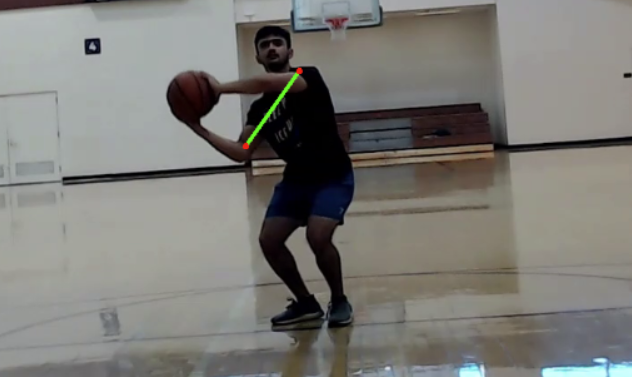
\includegraphics[width=0.40\textwidth]{imgs/openpose_bad.png}
  \caption{OpenPose Pose Detection}
  \label{fig:openpose}
\end{figure}

\begin{figure}[h]
  \centering
  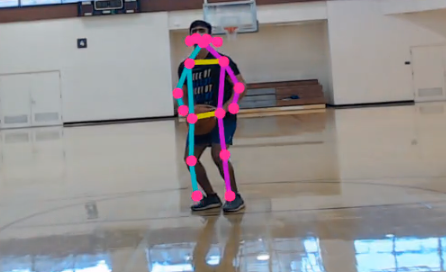
\includegraphics[width=0.40\textwidth]{imgs/movenet_good.png}
  \caption{MoveNet Pose Detection}
  \label{fig:movenet}
\end{figure}

\subsection{Feature Vector Generation}
Before we can train a classification model to predict the outcome of a shot in a video clip, we need to define how
we are going to generate the feature vectors for each video clip. 

As stated previously, we first want to downsample the video to reduce the number
of frames we are processing, as many of the frames will be redundant. Our initial approach was to
downsample the video by taking every nth frame, where n is a hyperparameter. However, we soon realized
that our clips were not all the same length, which would mean we would receive an inconsistent number of
frames per clip, which could potentially lead to dimensionality issues when we created our feature vectors, depending on our approach.
To solve this, we decided to take an absolute number of frames per clip, which we decided to be 60.

After downsampling, we perform pose estimation on each frame of the video clip. Using the pose estimation data, we defined two possible apporaches
to feature generation:
\begin{enumerate}
  \item Concatenate the pose estimation data from each frame of the clip into a single feature vector.
  \item Use the pose estimation data from each frame of the clip to generate a feature vector for each frame, and perform majority voting the feature vectors to generate the final prediction.
\end{enumerate}

Our pose estimator generates a set of 17 two dimensional coordinates, $S=\{(x_1, y_1), (x_2, y_2), \dots, (x_{17}, y_{17})\}$, where each coordinate $(x_i, y_i)$ is the
position on the image of keypoint $i$. For both approaches on each frame $i$, we concatenate all the coordinates to create a feature vector $v_{ij} \in \mathbb{R}^{34}$, where $v_{ij}$ is
a feature vector for frame $j$ of clip $i$. For our first approach, we take all the feature vectors for a single clip and concatenate them together, as seen in Figure \ref{fig:feature_vector}.
This takes 60 feature vectors of 34 dimensions and creates a feature vector $v_i \in \mathbb{R}^{2040}$, where $v_i$ is the feature vector for clip $i$. In contrast, for our second approach, we treat
each feature vector as a separate data point, and we perform a form of majority voting at the classification stage to generate our final prediction. Both of these approaches were tested, and performance
scores were generated.

\begin{figure}
  \centering
  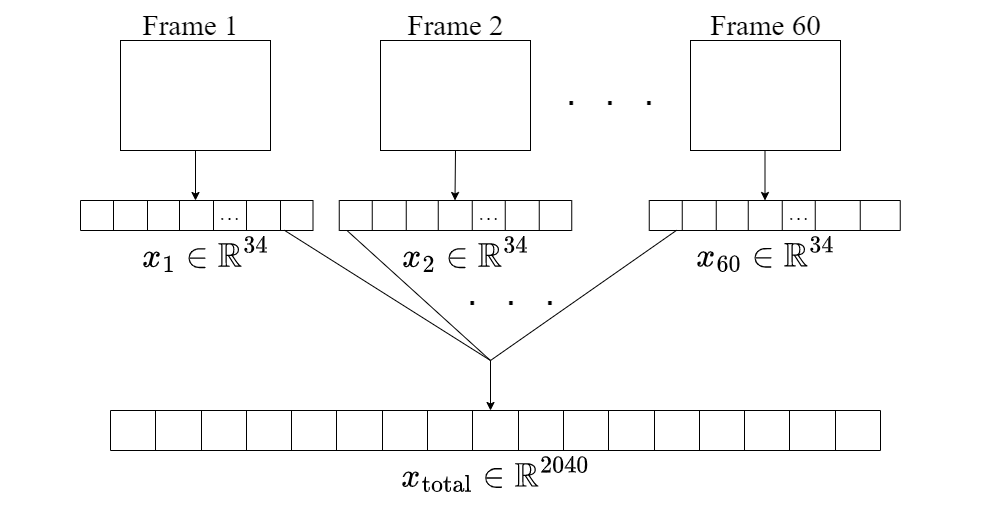
\includegraphics[width=0.45\textwidth, height=0.27\textwidth]{imgs/concat_vectors.png}
  \caption{First Approach to Feature Vector Generation}
  \label{fig:feature_vector}
\end{figure}

\subsection{Classification Model}
After we have generated our feature vectors, we used these vectors to train a classification model. We tested various classifiction models such as
Gradient Boosted Trees (Catboost), Support Vector Machines, Multi-Layer Perceptrons, and K Nearest Neighbors \cite{catboost}\cite{inproceedings}\cite{MURTAGH1991183}. We
did preliminary testing on the classification models by measuring the performance of each model on our first feature vector approach as a means of 
choosing the best model for us to do a deeper dive on. To measure the performance of each model, we used accuracy, as generating the AUC score was not 
feasible for some of the models. Table \ref{tab:table1} shows us the results of each model we tested:
\begin{table}[h]
  \begin{center}
    \caption{Accuracy Scores for Classification Models}
    \label{tab:table1}
    \begin{tabular}{l | r}
      \textbf{Model} & \textbf{Accuracy} \\
      \hline
      Catboost Gradient Boosting Tree & 0.636 \\
      Support Vector Machine & 0.580 \\
      Multi-Layer Perceptron & 0.556 \\
      K Nearest Neighbors & 0.602 \\
    \end{tabular}
  \end{center}
\end{table}

From the results, we see that the Catboost model got the highest accuracy score. As a result, we chose this model to perform the rest of our experiments on.

\section{Results}
In this section, we present and discuss in detail the results of our experiments. In all of these experiments, we used MoveNet as our pose estimator and Catboost
Gradient Boosting Tree as our classification model, as explained in the previous section.
\subsection{First Approach to Feature Vector Generation}
In our first experiment, we did a more extensive test on our first approach to feature vector generation. In our preliminary test,
we did not use our full set of data, as we generated more data after this preliminary experiment. Additionally, we would like to evaluate
the model on ROC-AUC score. Lastly, as we repeatedly retrained and reevaluated the model, we were getting performance scores that varied 
to some extent. Because of this, we decided to create a sample distribution of ROC-AUC scores we achieved for each iteration of our model. To do this,
we ran our model 100 times, each with a randomized train-test split. We then recorded each ROC-AUC score and plotted the histogram of the scores.
Figure \ref{fig:rocauc1} shows the distribution of our ROC-AUC scores for our first approach to feature generation.

% insert figure here
\begin{figure}[h]
  \centering
  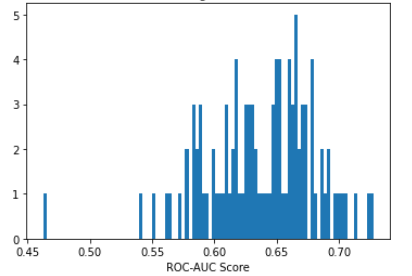
\includegraphics[width=0.45\textwidth]{imgs/approach1_rocauc.png}
  \caption{Distribution of ROC-AUC Scores for First Approach to Feature Vector Generation}
  \label{fig:rocauc1}
\end{figure}
We produced a mean ROC-AUC score of 0.638, with a standard deviation of 0.043. We also produced a histogram distribution of our accuracy scores, and
this distribution can be seen in Figure \ref{fig:accuracy1}.
% insert figure here
\begin{figure}[h]
  \centering
  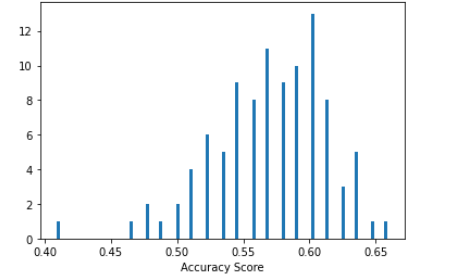
\includegraphics[width=0.45\textwidth]{imgs/approach1_acc.png}
  \caption{Distribution of Accuracy Scores for First Approach to Feature Vector Generation}
  \label{fig:accuracy1}
\end{figure}
We produced a mean accuracy score of 0.570, with a standard deviation of 0.044.

From these results, we see a performance that is better than random guessing, but not by much. Additionally, there is some 
nontrivial amount of deviation in the performance.

\subsection{Second Approach to Feature Vector Generation}
In our second experiment, we performed extensive performance tests on our second approach to feature generation. Firstly, we wanted
to see how effective our classification model would be classifying each frame of every video clip independently as a make or miss.
This meant we had to label each feature vector for each frame as a make or miss, depending on what the outcome of the clip it originated from.
We then trained our classification model on this data and evaluated its performance. Like we did before, we ran our model 100 times, each with a randomized train-test split
and generated a distribution of accuracy scores. We can see the results in Figure \ref{fig:frame_class_results}. From this distribution, we can see that our classification model
does fairly well in classifying each frame as part of a make clip or a miss clip. 

With this in mind, we decided that we could improve performance of predicting the outcome of each clip
by training the model on singular frames and producing our final prediction by performing some form of a majority vote on each frame for a given clip. This means, to predict the outcome of
a certain clip, we would input the 60 associated feature vectors into the model foe each frame. We predict the outcome for each of these frames, and if at least half of the frames
predict a make, our final output will be a make. If at least half of the frames predict a miss, our final output will be a miss. 

\begin{figure}
  \centering
  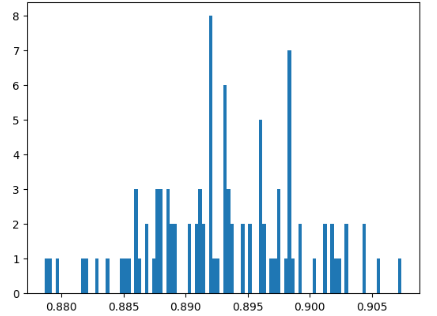
\includegraphics[width=0.45\textwidth]{imgs/frame_class_results.png}
  \caption{Distribution of Accuracy Scores for Frame Classification}
  \label{fig:frame_class_results}
\end{figure}

We ran this pipeline 100 times to generate a distribution of ROC-AUC scores and accuracy scores. These can be seen in Figure \ref{fig:rocauc2} and Figure \ref{fig:accuracy2} respectively.

\begin{figure}[h]
  \centering
  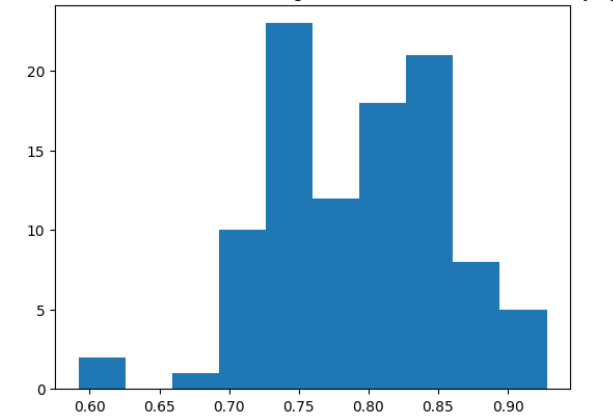
\includegraphics[width=0.45\textwidth]{imgs/equal_bias_roc.png}
  \caption{Distribution of ROC-AUC Scores for Equal Weighted Majority Voting}
  \label{fig:rocauc2}
\end{figure}

\begin{figure}[h]
  \centering
  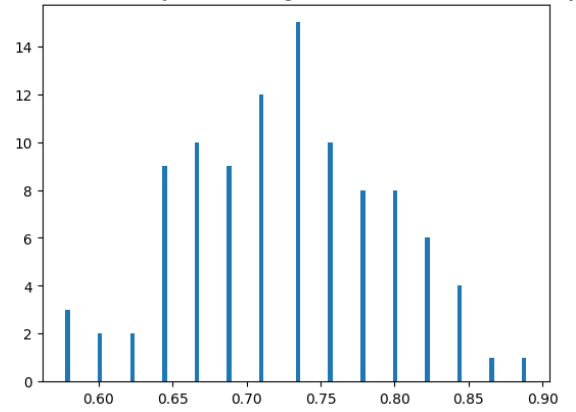
\includegraphics[width=0.45\textwidth]{imgs/equal_bias_acc.png}
  \caption{Distribution of Accuracy Scores for Equal Weighted Majority Voting}
  \label{fig:accuracy2}
\end{figure}

We achieved a mean ROC-AUC score of 0.794 with a standard deviation of 0.063 and a mean accuracy score of 0.726
with a standard deviation of 0.068. Though the standard deviation is slightly higher, the overall performance of this approach seems
to be much better than our first approach, with both ROC-AUC and accuracy scores increasing significantly.

\subsection{Tuning the Majority Voting Threshold}
After evaluating majority voting with equal weights, we wanted to see if we could improve the performance of this by tuning the threshold of our majority vote. We tried three different thresholds: 0.25, 0.5, and 0.75. For 
each threshold we, again, ran 100 iterations and generated a distribution of ROC-AUC scores and accuracy scores. The statistics of the distributions for each of the thresholds can be seen in Table \ref{tab:table2} and Table \ref{tab:table3}.

\begin{table}
  \begin{center}
    \begin{adjustbox}{width=0.47\textwidth}
    \begin{tabular}{|c|c|c|}
      \textbf{Threshold} & \textbf{Mean of ROC-AUC} & \textbf{Standard Deviation of ROC-AUC} \\
      \hline 
      0.25 & 0.795 & 0.067  \\
      0.50 & 0.794 & 0.063  \\
      0.75 & 0.793 & 0.058  \\
    \end{tabular}
    \end{adjustbox}
    \caption{Statistics of ROC-AUC Majority Voting Threshold Experiments}
    \label{tab:table2}
  \end{center}
\end{table}
\begin{table}
  \begin{center}
    \begin{adjustbox}{width=0.47\textwidth}
    \begin{tabular}{|c|c|c|}
      \textbf{Threshold} & \textbf{Mean of Accuracy} & \textbf{Standard Deviation of Accuracy} \\
      \hline 
      0.25 & 0.679 & 0.072  \\
      0.50 & 0.726 & 0.068  \\
      0.75 & 0.688 & 0.062  \\
    \end{tabular}
    \end{adjustbox}
    \caption{Statistics of Accuracy Majority Voting Threshold Experiments}
    \label{tab:table3}
  \end{center}
\end{table}

We see that the mean ROC-AUC score is highest for a threshold of 0.25, but only by a very small margin. In general, the ROC-AUC scores are quite similar, but it is clear
that when measuring performance by accuracy, the threshold of 0.5 tends to perform the best. The combination of the ROC-AUC scores and accuracy scores lead us to believe that
the threshold of 0.5 is the best choice.

\subsection{Modifying Majority Voting Criteria}
Our final experiment was to see if we could improve performance of the majority voting by using the median of the soft probability scores instead of the mean. This was done in
an attempt to reduce the effect of outliers on the vote. Again, we ran this 100 times and generated a performance score distribution. We attempted to use three different thresholding
values for this as well. The statistics of the ROC-AUC scores and accuracy scores

\begin{table}[h]
  \begin{center}
    \begin{adjustbox}{width=0.47\textwidth}
    \begin{tabular}{|c|c|c|}
      \textbf{Threshold} & \textbf{Mean of ROC-AUC} & \textbf{Standard Deviation of ROC-AUC} \\
      \hline 
      0.25 & 0.783 & 0.057  \\
      0.50 & 0.798 & 0.053  \\
      0.75 & 0.793 & 0.059  \\
    \end{tabular}
    \end{adjustbox}
    \caption{Statistics of ROC-AUC Median Voting Threshold Experiments}
    \label{tab:table4}
  \end{center}
\end{table}
\begin{table}[h]
  \begin{center}
    \begin{adjustbox}{width=0.47\textwidth}
    \begin{tabular}{|c|c|c|}
      \textbf{Threshold} & \textbf{Mean of Accuracy} & \textbf{Standard Deviation of Accuracy} \\
      \hline 
      0.25 & 0.688 & 0.057  \\
      0.50 & 0.733 & 0.054  \\
      0.75 & 0.663 & 0.078  \\
    \end{tabular}
    \end{adjustbox}
    \caption{Statistics of Accuracy Median Voting Threshold Experiments}
    \label{tab:table5}
  \end{center}
\end{table}

From this, we see that a threshold value of 0.5 for the median voting performs marginally better, but not significantly
enough to make a real difference.

\subsection{Other Explorations}
After achieving these results, we explored other methods that have historically been useful in improving the performance of
classification models. Principal Component Analysis (PCA) was the first method we explored to attempt to find the most significant
features of our features. However, when we performed the PCA transform, we greatly hindered the performance of our model to about the
performance of random guessing.

Additionally, we attempted stacking models together to improve our performance. We stacked many different classification models together
and attempted to use the majority voting method to improve the performance. However, this also hindered the performance of our model. 

\section{Analysis}
\subsection{Performance Analysis}
From our experiments we concluded that our second approach to feature generation and classification was
far more successful than our first approach. We believe that the main issue with our first approach was
insufficient data. We were only able to generate about 300 total clips, which meant we had about 210
feature vectors to train on and 90 to test on. This simply was not enough data to train a robust classifier.

When we trained the model on all the frames, we had a much larger dataset to train on, as each clip would give us 60
feature vectors. This gives the model more of a chance to learn patterns in the data to make its predictions. 

A deeper dive into our second approach to feature vector generation shows us that a threshold of 0.50 for the majority vote
performs the best, and a median vote goes not significantly change the performance.

\subsection{Pitfalls and Issues}
Although we were able to achieve adequate performance metrics with our approach, there are still some issues that
our current method cannot overcome.

\subsubsection{Invariance to Camera Position}

One of the main issues with our current approach is that our feature vector generation highly sensitive to the position of our camera. For our data collection,
we held the camera in a fixed position to record our test subject shooting free throws, and our feature vectors used the absolute coordinates of each of the 17 key points
to create our feature vector for a frame. This means that if we were to move the camera, or even if the person were to move, the feature vectors would be completely different, 
even if the shooting form is the same.

In order to fix this issue, we could use relative coordinates, fixing one of the key points as the origin, and calculating the relative coordinates of the other 16 key points.
This would allow our feature representation to be more invariant to the position of the camera or the test subject. Additionally, we could use a feature representation that took into
account the angles between the key points because the angles of joints are very important in determining the form of a shot. Using the angles would also make the feature representation
not depend on the absolute position.

\subsubsection{Loss of Temporal Information}

In our current representation, we are performing a majority vote on all the frames of a clip, but when we do this, we lose all temporal information and the sequential nature of the shot.
This means, theoretically, we could shuffle the frames of the clip, or even reverse the video, and the model will still predict the same. 

In order to capture the sequential
nature of the shooting form, it would have been beter to potentially use a recurrent neural network to capture the temporal information. 

\section{Conclusion and Future Works}
In this paper, we attempted to leverage pose estimation to help predict the outcome of a free throw. This involved collecting data
of a test subject shooting free throws, and using the pose estimation to generate feature vectors, and training a 
classification model to predict the outcome of a shot.

Through this process, we learned a great deal about how pose estimation works and the methodology behind generating feature vectors from data as well as
the nuances of training classification models.

Future works for this project would be to imrpove the robustness of our feature vector generation and capturing the temporal information, as explained 
in the previous section. Additionally, we could explore extending this project to work at different locations on the court and for different people shooting.
Lastly, we could explore the possibility of performing the prediction in real time, so that the results can be produced live instead of from a video recording.




%%%%%%%%% REFERENCES
{\small
\bibliographystyle{ieee_fullname}
\bibliography{egbib}
}

\end{document}

